\documentclass[english,usenames,dvipsnames]{beamer}
\usetheme{default}
\beamertemplatenavigationsymbolsempty
\setbeamertemplate{footline}[frame number]
\setbeamercolor{alerted text}{fg=blue1}
%\setbeamercolor{frametitle}{fg=blue2}
\usepackage[utf8]{inputenc}
\usepackage{caption}
\usepackage{booktabs}
\usepackage{appendixnumberbeamer}
\usepackage{babel}
\usepackage{amsmath}
\usepackage{hyperref}
\usepackage{geometry}
\usepackage{bbm}
\usepackage{amsthm}
\usepackage{verbatim}
%\usepackage{palatino}
\definecolor{red1}{RGB}{255,50,0}
\definecolor{blue1}{RGB}{80,80,255}
\definecolor{blue2}{rgb}{0.22,0.37,1}
\definecolor{green1}{RGB}{34,139,35}

\setbeamertemplate{itemize items}[default]


\title{Employee Spinouts, Creative Destruction and Endogenous Growth}
\author{Nicolas Fernandez-Arias}
\institute{Student Macro Workshop}
\date{March 7, 2019}

\begin{document}

\maketitle

%%% TO DO

%%% 
%%% (1) Put QUESTION i want to answer in MOTIVATION - i.e., should we encourage or discourage more spnout formation?
%%%%
%%%% (2) Shorten - need to put a few more slides in the appendix.

\begin{frame}{Motivation}
\begin{itemize}
	\item Question: should we encourage or discourage employee spinouts? 
	\begin{itemize}
		\item Spinouts = firms founded by ex-employees
	\end{itemize}
	\item Entry contributes significantly to productivity growth
	\begin{itemize}
		\item Over 10-year horizon, 25\% of labor productivity growth accounted by entry in manufacturing (Baily-Bartelsman-Haltiwanger 1996)
		\item ~25\% of aggregate productivity growth due to entrants (Akcigit-Kerr 2017)
	\end{itemize}
	\item Spinouts are most innovative entrants
	\begin{itemize}
		\item Fairchild semiconductor / Silicon Valley (Saxenian 1994); Detroit automakers
		\item Spinouts: more patents / R\&D, sales growth, survival (Baslandze 2019) 
		\item Spinouts 15-30\% of entrants; larger, grow faster, more survival (Muendler et al. 2012, Brazilian data)
	\end{itemize}
\end{itemize}
\end{frame}

\begin{frame}{Motivation - Theory}
\label{theory_big_picture}
\begin{itemize}
	\item Schumpeter 1942, Arrow 1962, Romer 1986, Grossman-Helpman 1991, etc.: \alert{underinvestment} in knowledge due to \alert{limited excludability}
	\item Patent literature: dynamic efficiency vs. static monopoly distortion tradeoff
	\item Creative destruction by spinouts similar tradeoff
	\item Should we encourage or discourage spinout formation?
	\item Existing frameworks (e.g., Franco-Filson 2006, Baslandze 2019) underemphasize disincentive for firm R\&D 
\end{itemize}
\end{frame}

\begin{frame}{Related literature}
\begin{itemize}
	\item Firm dynamics and endogenous growth
	\begin{itemize}
		\item Romer 1986, Grossman \& Helpman 1991, Aghion \& Howitt 1992, Klette \& Kortum 2004, Acmemoglu \& Akcigit 2012, Akcigit \& Kerr 2017
	\end{itemize}
	\item Models of employee spinouts
	\begin{itemize}
		\item Klepper 2002, Klepper \& Sleeper 2005, Franco \& Filson 2006, Franco \& Mitchell 2008, Rauch 2015, Rossi-Hansberg \& Chatterjee 2012
		\item Baslandze 2019: closest, but spinouts \alert{do not directly compete} with parents
	\end{itemize}
	\item Empirics on employee mobility, spinouts
	\begin{itemize}
		\item Spawning of spinouts: Gompers et al. 2005, Garmaise 2011, Baslandze 2019
		\item Effect on parent firms: Campbell et. al 2012, Wezel et al. 2006
		\item Effect of non-compete enforcement: Garmaise 2009, Marx et al 2009, Samila-Sorenson 2011, Jeffers 2018
	\end{itemize}
\end{itemize}
\end{frame}

%\begin{frame}
%\frametitle{Table of Contents}
%	\tableofcontents
%\end{frame}

\section{Model}

\subsection{Description}

\begin{frame}{Model - Overview}
\begin{itemize}	
	\item Builds on (nests) standard \alert{quality ladders model} of \alert{endogenous growth} through \alert{creative destruction} 
	\begin{itemize}
		\item Built most closely on Akcigit-Kerr 2017, "Growth through heterogeneous innovations"
		\item Offshoot of Grossman-Helpman 1991
	\end{itemize}
	\item \textbf{New feature:} R\&D workers \alert{learn on the job} how to form \alert{competing spinouts}
	\begin{itemize}
		\item Creates \alert{endogenous knowledge spillovers} \ldots
		\item \ldots but also may \alert{disincentivize incumbent R\&D}
	\end{itemize} 
\end{itemize}
\end{frame}

\begin{frame}{Model - Households}
\begin{itemize}
	\item Unit continuum of households are risk-neutral (tractability), discount rate $\rho > 0$, objective
	\begin{align*}
		\mathbb{E}_t \int_0^{\infty} e^{-\rho s} c_i(t+s) ds
	\end{align*}
	where $c_i(t)$ is household $i$ consumption of final good at time $t$
	\item Unit endowment of labor, supplied inelastically to final goods production, intermediate goods production or R\&D
\end{itemize}
\end{frame}

\begin{frame}{Model - Production}
\begin{itemize}
	\item Final good
	\item Continuum of intermediate goods
	\item Improving intermediate goods through innovation
\end{itemize}
\end{frame}


\begin{frame}{Model - Final good}
\begin{itemize}
	\item Final good output $Y(t)$,
	\begin{align*}
		Y(t) &= \frac{L_F^{\beta}(t)}{1-\beta} \int_0^1 q_j^{\beta}(t) k_j^{1-\beta} (t) dj 
	\end{align*}
	\item Labor $L_F(t)$
	\item Intermediate goods $k_j(t)$, qualities $q_j(t)$, $j \in [0,1]$
\end{itemize}
\end{frame}

\begin{frame}{Model - Intermediate goods}
\begin{itemize}
	\item Production technology
	\begin{align*}
		k_j = Q l_j
	\end{align*}
	where $Q = \int_0^1 q_j dj$ is average quality
	\item Scaling to ensure balanced growth
	\item Based on setup in AK 2017
\end{itemize}
\end{frame}

\begin{frame}{Model - Innovation}
\begin{itemize}
	\item R\&D by incumbents, potential entrants and potential spinouts 
	\item Innovation in good $j$ yields temporary monopoly on good $j$
	\item Quality jumps to $\lambda q_j$, for $\lambda > 1$
\end{itemize}
\end{frame}

\begin{frame}{Model - R\&D by incumbents}
\begin{itemize}
	\item Incumbent with quality $q$ hires $\big(\frac{q}{Q}\big)z_I$ units of R\&D labor
	\item Discovers next innovation with Poison intensity
	\begin{align*}
		\tau^I &= \chi_I z_I \phi_I(z_I) 
	\end{align*}
	where $\phi_I(z) = z^{-\psi_I}$
	\item Baseline $\psi = 0.5$ corresponds to quadratic cost function
	\item DRS captures \alert{fishing out} of ideas
\end{itemize}
\end{frame}

% Rename these slides in parallel ie R&D by entrants / spinouts, etc.

\begin{frame}{Model - R\&D by potential entrants \& spinouts}
\begin{itemize}
	\item Each good line $j$,
	\begin{itemize}
		\item Unit mass of ordinary \alert{potential entrants} owned by households in aggregate
		\item Mass $m_j$ of \alert{potential spinouts} owned by individual households
	\end{itemize}
	\item Individual effort of potential entrant $e$ and potential entrant $s$ (suppressing $j$): $z_E^e, z_S^s$ 
	\item Aggregate: 
	\begin{align*}
		z_E &= \int_0^1 z_E^e de \\
		z_S &= \int_0^m z_S^s ds 
	\end{align*}
	\item When innovation occurs, \alert{$m$ jumps to 0}
\end{itemize}
\end{frame}


\begin{frame}{Model - R\&D by potential entrants \& spinouts}
\begin{itemize}
	\item Potential entrants and spinouts individually hire $\big(\frac{q}{Q}\big)z$ for $z$ units of R\&D effort and arrival rate  
	\begin{align*}
	\tau^k &= \chi_{k} z \phi_{SE} (z_E + z_S)
	\end{align*}
	for $k \in \{E,S\}$, $\phi_{SE}(z) = z^{-\psi_{SE}}$
	\item Potential spinouts have \alert{capacity constraint} $z_S^s \le \xi$
	\item Aggregate DRS captures
	\begin{itemize}
		\item \alert{redundant} research
		\item fishing out of ideas
	\end{itemize} 
	\item \alert{Different pool of ideas} from incumbent (tractability, some realism)
\end{itemize}
\end{frame}

\begin{frame}{Model - Formation of potential spinouts}
\begin{itemize}
	\item At rate $\Big(\frac{q_j}{Q}\Big)^{-1} \nu l_{ij}^{RD}$ worker $i$ gets idea from for potential spinout on line $j$
	\item Immediately begins hiring R\&D 
	\begin{itemize}
		\item Continue to work - no opportunity cost (tractability) 
		\item Can interpret as selling, for full value, to competitive investor fringe owned by households
	\end{itemize}
	\item Law of motion for mass of potential spinouts $m_j$  
	\begin{align*}
		\dot{m}_j &= \overbrace{\alert{\Big(\frac{q_j}{Q}\Big)^{-1}} \nu}^{\textrm{Idea generation rate}} \times \overbrace{\alert{\Big(\frac{q_j}{Q}\Big) }(z_{I,j} + z_{E,j} + z_{S,j})}^{\textrm{R\&D employoment}} \\
		                    &= \nu (z_{I,j} + z_{E,j} + z_{S,j})
	\end{align*}
\end{itemize}
\end{frame}

\begin{frame}{Model - Aggregation}
\begin{itemize}
	\item $\tilde{q} = q/Q_t$
	\item $\mu(\tilde{q},m,t)$ time-varying distribution of product lines in $(\tilde{q},m)$-space 
	\item $\tau(\tilde{q},m,t) = \sum_{K \in \{I,E,S\}} \tau^K(\tilde{q},m,t)$
	\item Growth rate of $Q_t$
	\begin{align*}
		g_t &= (\lambda -1) \int_{\tilde{q},m} \tilde{q} \tau(\tilde{q},m,t) \mu(\tilde{q},m,t) d\tilde{q}dm
	\end{align*}
\end{itemize}
\end{frame}


\subsection{Equilibrium}

%%
%% Need to SIGNIFINCANTLY fix this slide, but not a priority. Still should be easy
% because you are overthinking it - just define what an equilibrium is (i.e., everyone optimizes)
% you don't have to show the necessary conditions of optimization.

%% Also, will probably just show this slide quickly and skip over during the presentation because
% not much time.

\begin{frame}{Equilibrium - Defnition}
\begin{itemize}
	\footnotesize 
	\item Interest rate $r(t)$, final goods wage $w_F(t)$, intermediate goods wage $w_I(t)$, R\&D wage $w(\tilde{q},m,t)$, household consumption and labor supply, individual non-incumbent R\&D effort $\{z_E^e(\tilde{q},m,t)\}_{e \in [0,1]},\{z_S^s(\tilde{q},m,t)\}_{s \in [0,m]}$, product-line-level R\&D efforts $z_K(\tilde{q},m,t)$ for $K \in \{I,E,S\}$, prices and quantities of intermediate goods $p(\tilde{q},m,t),k(\tilde{q},m,t)$, production of final good $Y(t)$, and distribution $\mu(\tilde{q},m,t)$ such that:
	\begin{itemize}
		\footnotesize
		\item Households optimize taking prices and the equilibrium value of knowledge as given
		\item Intermediate goods incumbents optimally price their output
		\item Final goods firms maximize profits taking prices as given
		\item Potential entrants and potential spinouts optimize R\&D taking innovation rates as given
		\item Incumbents optimize R\&D taking into account effect on innovation rate
		\item Product-line-level R\&D effort aggregates from individual policy functions
		\item Labor, bond and goods markets clear 
	\end{itemize}
\end{itemize}
\end{frame}

% This is in the wrong order - put this at the end, after talking about static / dynamic equilibrium conditions
%% Also - this is not "existence of BGP", it's something else - be more rigorous about what you're doing, 
% it's confusing.

\begin{frame}{Equilibrium - Static equilibrium conditions}
\begin{itemize}
	\item Given aggregate R\&D labor allocation $L^{RD}$
	\item $C(\beta) = \Big(\frac{\beta}{1-\beta} (1-\beta)^{\frac{1-\beta}{\beta}} \Big)^{\beta}$ 
	\item Final goods wage $w_F = C(\beta) Q$
	\item Intermediate goods price $p = (1-\beta)^{-1} \frac{w_F}{Q} = (1-\beta)^{-1} C(\beta)$
	\item Final goods production labor allocation $L_F = \frac{1 - L_{RD}}{1 + \frac{1-\beta}{C(\beta)}}$
	\item Intermediate goods firm profits $\beta q_j L_F$
\end{itemize}
\end{frame}

\begin{frame}{Equilibrium - Dynamic equilibrium conditions}
\begin{itemize}
	\item Worker indifference conditions
	\item Incumbent, potential spinout HJBs
	\item Potential entrants zero profit condition
\end{itemize}
\end{frame}

\begin{frame}{Equilibrium - Worker indifference conditions}
\begin{itemize}
	\item $w_I(t) = w_F(t) = \bar{w}(t)$
	\item $W(q,m,t)$ value of potential spinout
	\item $w(\tilde{q},m,t) + \tilde{q}^{-1} \nu W(q,m,t) = \bar{w}(t)$
	\item \alert{Paying for knowledge} as in Franco-Filson 2006
\end{itemize}
\end{frame}

\begin{frame}{Equilibrium - HJB equations}
\begin{itemize}
	\item Incumbent HJB
	\footnotesize
	\begin{align*}
	(r(t) + &\overbrace{\tau_{SE}(\tilde{q},m,t)}^{\textrm{Creative destruction}}) V(q,m,t) = \overbrace{\beta q L_F(t)}^{\textrm{Flow profit}} + \overbrace{a_{SE}(\tilde{q},m,t) \nu V_m(q,m,t)}^{\textrm{Drift in $m$-space due to $z_E,z_S$}} \\
	& + \overbrace{V_t(q,m,t)}^{\textrm{Non-stationarity}} + \max_{z \ge 0} \Big \{ \overbrace{\chi_I z \phi_I(z)\big[V(\lambda q,0,t) - V(q,m,t) \big] }^{\textrm{Innovation arrival}}\\
	& - \underbrace{\tilde{q}z w(\tilde{q},m,t) + \tilde{q}^{-1} \nu \tilde{q} z V_m(q,m,t)}_{\textrm{Effective R\&D cost}}\Big\}
	\end{align*}
	\normalsize
	\item Potential spinout HJB
	\footnotesize
	\begin{align*}
	(r(t) + \overbrace{\tau(\tilde{q},m,t)}^{\textrm{Innovation rate}}) &W(q,m,t) = \overbrace{a(\tilde{q},m,t) \nu W_m(q,m,t)}^{\textrm{Drift in $m$-space}} + \overbrace{W_t(q,m,t)}^{\textrm{Non-stationarity}} \\
	&+ \max_{0 \le z \le \xi} \Big \{ \overbrace{\chi_S z \phi_{SE}(z_E(\tilde{q},m,t) + z_S(\tilde{q},m,t)) V(\lambda q,0,t)}^{\textrm{Innovation arrival}} \\
	& - \underbrace{\tilde{q}z w(\tilde{q},m,t)}_{\textrm{R\&D cost}}\Big\}
	\end{align*}
\end{itemize}
\end{frame}

\begin{frame}{Equilibrium - Potential entrants free entry}
\begin{itemize}
	\item Free entry implies zero expected profits
	\begin{align*}
		\chi_E \phi_{SE}\Big(z_E(\tilde{q},m,t) + z_S(\tilde{q},m,t)\Big) V(\lambda q,0,t) \ge \tilde{q} w(\tilde{q},m,t)
	\end{align*} 
	with equality whenever $z_E(m) > 0$
	\item Gradually outcompeted by potential spinouts
	\item Product-line level potential spinout R\&D effort $z_S(\tilde{q},m,t)$
	\begin{itemize}
		\item $z_S(\tilde{q},m,t) = \xi m$ for $m \le M(\tilde{q},t)$
		\item $z_S(\tilde{q},m,t) = \xi M(\tilde{q},t)$ for $m > M(\tilde{q},t)$
		\item $M(\tilde{q},t)$ defined by $\chi_S \phi_{SE} (\xi M(\tilde{q},t)) V(\lambda \tilde{q},0,t) = \tilde{q} \bar{w}(t)$
	\end{itemize}
	\item $\chi_S \le \chi_E$: nests model with no spinouts, no state variable
\end{itemize}
\end{frame}

\begin{frame}[label = equilibrium_BGP]{Equilibrium - Balanced growth path (BGP)}
\begin{itemize}
	\item $Q(t) = \int_0^1 q_{jt} dj$, $Y(t),w_I(t),w_F(t)$ grow exponentially at constant rate $g$
	\item $w(\tilde{q},m,t) = Q(t) w(m)$
	\item $z_K(\tilde{q},m,t) = z_K(m)$ for $K \in \{I,E,S\}$
	\item $r(t) \equiv r$
	\item $\hat{\mu}(m,t),E[\tilde{q}|m,t]$ constant in $t$ \hyperlink{BGP_stationary_distribution}{\beamergotobutton{details}}
	\item $M(\tilde{q},t) = M$ 
\end{itemize}
\end{frame}

%%% Put slide here about confirming the guess
\begin{frame}[label=confirming_bgp]{Equilibrium - BGP guess and verify}
\begin{itemize}
	\item Guess and verify 
	\item Guess innovation rates and wages depend only on $m$
	\item HJBs confirm policies depend only on $m$ \hyperlink{incumbent_BGP}{\beamergotobutton{incumbent}} \hyperlink{spinout_BGP}{\beamergotobutton{potential spinout}}
	\item This confirms existence of stationary distribution $\mu(m)$ \hyperlink{mu_details}{\beamergotobutton{details}}
	\item Constant $E[\tilde{q}|m,t] = \gamma(m)$ confirms constant growth rate and labor allocations \hyperlink{gamma_details}{\beamergotobutton{computing $\gamma(m)$}} \hyperlink{aggregation_BGP}{\beamergotobutton{aggregation}}
\end{itemize}
\end{frame}

\subsection{Solution}

\begin{frame}{Solving the model}
\begin{enumerate}
	\small
	\item Guess $g, L_{RD}, w(m)$
	\begin{enumerate}
		\small
		\item Compute $L_I,L_F,\pi$ using static equilibrium conditions given $L_{RD}$ 
		\item Guess $z_S(m),z_E(m)$ 
		\begin{enumerate}
			\small
			\item Solve incumbent HJB for $V(m),z_I(m)$ given $z_S(m),z_E(m),\pi,w(m)$
			\item Update $z_S(m),z_E(m)$ using free entry conditions (taking previous guess as given) and check convergence, if not converged go back to 1.2.
		\end{enumerate}
		\item Solve spinout HJB for $W(m)$ given $z_S(m),z_E(m),z_I(m),V(m),w(m)$
		\item Compute implied $w(m)$ given $W(m)$ and worker indifference condition
		\item Aggregate to compute $\mu(m)$ and $\gamma(m)$ (needed $g$ guess because $\gamma(m)$ depends on $g$)
		\item Aggregate to compute $L_{RD}$ and $g$ given $\mu(m),\gamma(m),\tau(m)$
		\item Update $g,L_{RD},w(m)$, check convergence, if not converged go back to 1.
	\end{enumerate}
\end{enumerate}
\end{frame}

\section{Calibration}

\begin{frame}{Calibration - Parameters}
	\begin{table}[h]
		\footnotesize
		\centering{}%
		\begin{tabular}{lll}
			Table 1 &  &  \tabularnewline
			Calibration Parameters &  &  \tabularnewline
			\hline 
			Parameter & Explanation & Value\tabularnewline
			\tabularnewline
			\hline 
			Normalized & & \tabularnewline
			$\xi$ & Spinout R\&D capacity & 10 \tabularnewline
			&  & \tabularnewline
			Chosen outside model & & \tabularnewline
			$\psi_I$ & Incumbent R\&D curvature & 0.5\tabularnewline
			$\psi_E$ & non-Incumbent R\&D curvature & 0.5\tabularnewline
			&  & \tabularnewline
			Chosen to match data & & \tabularnewline
			$\rho$ & Discount rate & 0.05\tabularnewline
			$\beta$ & $\beta^{-1}$ is EoS between intermediate goods & 0.106\tabularnewline
			$\lambda$ & Innovation step size & 1.053\tabularnewline
			$\chi_I$ & Incumbent R\&D productivity & 3.252\tabularnewline
			$\chi_E$ & Entrant R\&D productivity & 1.203\tabularnewline
			$\chi_S$ & Spinout R\&D productivity & 1.425\tabularnewline
			$\nu$ & Learning rate & 0.0103
		\end{tabular}
	\end{table}
\end{frame}

\begin{frame}{Calibration - Targets}
	\begin{table}[H]
		\footnotesize
		\centering{}%
		\begin{tabular}{lll}
			Table 2 &  &  \tabularnewline
			Calibration Targets &  &  \tabularnewline
			\hline 
			Moment  & Target & Model \tabularnewline
			&   & \tabularnewline
			\hline 
			Growth rate $g$ & 0.015 & 0.0198 \tabularnewline
			Risk-adjusted interest rate $r$ & 0.05 & 0.05 \tabularnewline
			Profit / sales ratio & .109 & .109 \tabularnewline
			R\&D spending / sales ratio & 0.15 & 0.093
			\tabularnewline
			Internal patent share & 0.2 & 0.202
			\tabularnewline
			Spinout entry rate & 0.05 & 0.084
			\tabularnewline
			Share of creative destruction by spinouts & 0.30 & 0.283 
		\end{tabular}
	\end{table}
\end{frame}

\subsection{Visualizing Equilibrium}

% Make sure tell the audience exactly what they're supposed to take away from each chart
% don't just "prove you solved the model" - be clear that it's about showing what an equilibrium
% looks like, and showing the comparative statics.

\begin{frame}[label = innovation_rates]{Calibration - Innovation rates}\hyperlink{incumbent_value}{\beamergotobutton{Incumbent Value}} \hyperlink{spinout_value}{\beamergotobutton{Spinout Value}} \hyperlink{stationary_distribution_m}{\beamergotobutton{$\mu(m),\gamma(m)$}} \hyperlink{stationary_distribution_t}{\beamergotobutton{$\mu(t),\gamma(t)$}}
\begin{figure}
	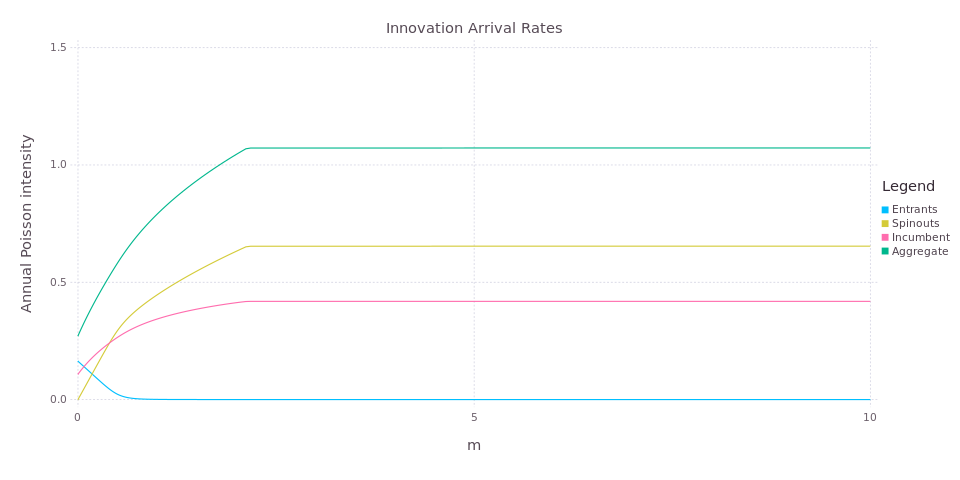
\includegraphics[scale=0.3]{../code/julia/figures/presentation/innovation_rates.png}
\end{figure}
\end{frame}

\begin{frame}{Calibration - R\&D wage}
\begin{figure}
	\includegraphics[scale=0.33]{../code/julia/figures/presentation/plot_effectiveRDWage_vs_t.png}
\end{figure}
\end{frame}

\subsection{Comparative statics}

\begin{frame}{Comparative statics $\nu \xi, \chi_S$: R\&D, growth response}
\begin{figure}
	\includegraphics[scale=0.33]{../code/julia/figures/presentation/nuxi_chiS_g_plot_2.png}
\end{figure}
\end{frame}

\begin{frame}{Comparative statics $\nu \xi$: R\&D, growth decompositions}
\begin{figure}
	\includegraphics[scale=0.31]{../code/julia/figures/presentation/nuxi_RDandGrowth_plot.png}
\end{figure}
\end{frame}

\begin{frame}{Comparative statics $\nu \xi , \chi_S$: Welfare}
\begin{figure}
	\includegraphics[scale=0.3]{../code/julia/figures/presentation/nuxi_chiS_welfare_plot.png}
	\footnotesize
	\begin{align*}
	\textrm{Welfare} &= \int_0^{\infty} e^{-\rho t} Y(t|Q_0 = 1) dt = \frac{Y(0|Q_0 = 1)}{\rho - g}
	\end{align*}
\end{figure}
\end{frame}






\section{Empirics (proposal)}

\subsection{Data}

\begin{frame}{Empirics - Data}
\begin{itemize}
	\item Compustat / CRSP
	\item Venture Source database on venture-capital investments in the US since 1986
	\item Crunchbase (free version)
	\item NBER USPTO patent database
	\item State- and federal R\&D subsidies in Bloom et al 2013 (updated in 2017)
	\item Star-Bishara-Prescott 2019 state-level non-compete enforceability
	\item Jeffers 2018 state-level non-compete enforcement changes
\end{itemize}
\end{frame}

\subsection{Identifying spinouts}

\begin{frame}{Empirics - Identifying spinouts}
\begin{itemize}
	\item \alert{Founder biographies} in Venture Source: text field with information on \alert{previous employment}
	\item Match to Compustat by \alert{parent firm name}, as in Gompers et al. 2005, "Entrepreneurial spawning: ..." (same data set)
	\item Extension: Match to NBER-USPTO patent database by \alert{employee name $\times$ parent firm name} to get closer information on dates of previous employment (as in Baslandze 2019)
\end{itemize}
\end{frame}

\subsection{Effect of R\&D on spinout formation}

\begin{frame}{Empirics - Estimating effect of R\&D on spinout formation}
\begin{itemize}
	\item Use \alert{state- and federal-level tax incentives for R\&D} to construct \alert{instruments for firm-level R\&D spending}
	\item Federal-level: firm-specific component from firm-specific history of R\&D
	\begin{itemize}
		\item Satisfies exclusion restriction, since firm-specific
		\item ...but may be \alert{low power}
	\end{itemize}
	\item State-level: more variation but fails exclusion restriction unless...
	\begin{itemize}
		\item Look at out of state spinouts (\alert{low power})
		\item Use model to interpret effects of state-level changes in R\&D subsidies (\alert{highly model-dependent})
	\end{itemize}
\end{itemize}
\end{frame}

\subsection{Effect of VC funding on parent firm market value}

\begin{frame}{Empirics - Estimating competition by spinouts}
\begin{itemize}
	\item Existing work on spinouts / growth does not emphasize creative destruction (e.g. Franco-Filson 2006, Baslandze 2019)
	\item Industry studies, e.g. Campbell et al. 2012 (legal services industry), Klepper-Sleeper 2005 (laser industry)
	\item Venture Source and Compustat / CRSP provide additional way to estimate:
	\begin{itemize}
		\item Measure competition \alert{via effect of dollar of VC funding on parent firm stock price}
		\item Regression discontinuity: VC funding discontinuously affects stock prices only through through news about future competition
		\item Or maybe IV design: state LP returns as IV for VC funding as in Samila-Sorensen 2011? Exclusion restriction?
		\item Need to \alert{extend model}: fraction $\zeta \in (0,1)$ of spinouts in different lines
	\end{itemize}
\end{itemize}
\end{frame}

\begin{frame}{Empirics - Validating the model}
\begin{itemize}
	\item Compare predictions to variation by state-level non-compete enforceability
	\item Extend model
	\begin{itemize}
		\item Easiest (e.g. Baslandze 2019): non-compete enforcement represented by fixed cost of spinout formation.
		\item Ideally: allow non-compete contracts to be signed in the model (simple contracts, e.g. permanent, should be tractable)
	\end{itemize}
\end{itemize}
\end{frame}

\appendix

\begin{frame}[label = incumbent_value]{Incumbent value and policy}\hyperlink{innovation_rates}{\beamergotobutton{back}}
\begin{figure}
	\includegraphics[scale=0.33]{../code/julia/figures/presentation/plot_V_zI.png}
\end{figure}
\end{frame}

\begin{frame}[label = spinout_value]{Potential spinout value and policy}\hyperlink{innovation_rates}{\beamergotobutton{back}}
\begin{figure}
\includegraphics[scale=0.33]{../code/julia/figures/presentation/plot_W_zSoverm.png}
\end{figure}
\end{frame}

\begin{frame}[label = stationary_distribution_m]{Stationary distribution}\hyperlink{innovation_rates}{\beamergotobutton{back}}
\begin{figure}
\includegraphics[scale=0.33]{../code/julia/figures/presentation/plot_mu_gamma_m.png}
\end{figure}
\end{frame}

\begin{frame}[label = stationary_distribution_t]{Stationary distribution vs $t$}\hyperlink{innovation_rates}{\beamergotobutton{back}}
\begin{figure}
\includegraphics[scale=0.33]{../code/julia/figures/presentation/plot_mu_gamma_t.png}
\end{figure}
\end{frame}


\begin{frame}[label = mu_details]{Equilibrium - Confirming the guess, $\mu(m)$ details}\hyperlink{confirming_bgp}{\beamergotobutton{back}}
\begin{itemize}
	\item $\mu(m)$ satisfies Kolmogorov Forward Equation
	\begin{align*}
	0 &= - a'(m)\mu(m) - a(m) \mu'(m) - \tau(m) \mu(m)
	\end{align*}
	implies $\mu(m) = C_{\mu} e^{-\int_0^m \frac{a'(m') + \tau(m')}{a(m')} dm'}$
	\item $C_{\mu}$ determined by $\int_0^{\infty} \mu(m) dm = 1$
\end{itemize}
\end{frame}

\begin{frame}[label = gamma_details]{Equilibrium - Confirming the guess, $\gamma(m)$ details}\hyperlink{confirming_bgp}{\beamergotobutton{back}}
\begin{itemize}
\item $s(m)$ is eq. time to reach state $m$
\begin{align*}
s(m) &= \int_0^{m} \frac{1}{a(m') \nu} dm'
\end{align*}
\item Given growth $g$, 
\begin{align*}
\tilde{\gamma}(s) = C_{\gamma} e^{-gs}
\end{align*}
\item $\gamma(m) = \tilde{\gamma}(s(m))$
\item $C_{\gamma}$ determined by $\int_0^{\infty} \gamma(m) \mu(m) dm = 1$
\footnotesize
\item Actually one more equation determining $C_{\gamma}$, but it is redundant
\begin{align*}
C_{\gamma} = \gamma(0) &= \lambda \int_0^{\infty} \gamma(m) \tau(m) \mu(m) dm
\end{align*}
\end{itemize}
\end{frame}

\begin{frame}[label = incumbent_BGP]{Equilibrium - Finding the BGP}\hyperlink{confirming_bgp}{\beamergotobutton{back}}
\begin{itemize}
	\item Guess and verify $V(q,m,t) = qV(m)$
	\footnotesize
	\begin{align*}
	(r + \tau_{SE}(m)) q V(m) &= \pi q + a_{SE}(m) \nu q V'(m) \\
	& + \max_{z \ge 0} \Big \{ z \phi_I(z) \big[\lambda q V(0) - q V(m) \big] \\
	& - \big(\frac{q}{Q_t}\big)z Q_t w(m) + \nu z q V'(m) \Big\}
	\end{align*}
	\normalsize
	\item Divide both sides by $q$ to get equation for $V(m)$
	\footnotesize
	\begin{align*}
	(r + \tau_SE(m)) V(m) &= \pi + a_{SE}(m) \nu V'(m) + \max_{z \ge 0} \Big \{ z \phi_I(z) \big[\lambda V(0) - V(m) \big] \\
	& - z w(m) + \nu z V'(m) \Big\}
	\end{align*}
\end{itemize}
\end{frame}

\begin{frame}[label = BGP_stationary_distribution]{Equilibrium - BGP stationary distribution}\hyperlink{equilibrium_BGP}{\beamergotobutton{back}}
\begin{itemize}
	\item Even on BGP, $\mu(\tilde{q},m,t)$ 
	\begin{itemize}
		\item \alert{Not constant over $t$}  
		\item Proportional growth + no exit for low $\tilde{q}$
	\end{itemize} 
	\item Existence only requires
	\begin{itemize}
		\item Constant marginal: $\int_0^{\infty} \mu(\tilde{q},m,t) d\tilde{q} \equiv \mu(m)$
		\item Constant conditional expectation: $E[\tilde{q} | m,t] \equiv \gamma(m)$ 
		\item This relies on risk-neutrality and no opportunity cost for potential spinout managers
	\end{itemize} 
\end{itemize}
\end{frame}

\begin{frame}[label = spinout_BGP]{Equilibrium - Finding the BGP}\hyperlink{confirming_bgp}{\beamergotobutton{back}}
\begin{itemize}
\item Potential spinout value $W(q,m,t) = qW(m)$ and satisfies 
\small
\begin{align*}
(r + \tau(m)) W(m) &= a(m) \nu W'(m) \\
&+ \max_{0 \le z \le \xi} \Big \{ z \phi_{SE}(z_S(m) + z_E(m)) \lambda V(0) - zw(m) \Big \}
\end{align*}
\end{itemize}
\end{frame}

\begin{frame}[label = aggregation_BGP]{Equilibrium - Aggregation}\hyperlink{confirming_bgp}{\beamergotobutton{back}}
\begin{itemize}
	\item Growth
	\begin{align*}
	g &= (\lambda - 1) \int_0^{\infty} \tau(m) \gamma(m) \mu(m) dm
	\end{align*}
	\item R\&D labor allocation
	\begin{align*}
	L_{RD} &= \int_0^{\infty} a(m) \gamma(m) \mu(m) dm 
	\end{align*}
\end{itemize}
\end{frame}

\section{Extensions}

\begin{frame}{Endogenous learning}
\begin{itemize}
	\item Workers learn at an exogenous rate in this model
	\item Instead, it could be posited that they have a technology for learning with some exogenous productivity, opening up an additional margin of adjustment
	\item Should be feasible, but not a particularly important extension
\end{itemize}
\end{frame}

\begin{frame}{Partial knowledge expiry}
\begin{itemize}
	\item In the baseline model, innovations immediately render spinouts' knowledge obsolete
	\item The model can be made more flexible by positing that an exogenous fraction $\theta$ of their knowledge becomes obsolete upon this event
	\item This does require a slightly different solution approach but should still be tractable
	\item This could be important because it frees up the strength of the ``escape competition'' effect of spinout entry on incumbent incentives for R\&D
\end{itemize}
\end{frame}

\begin{frame}{Non-competition agreements}
\begin{itemize}
	\item The most ambitious extension / application
	\item Good way to test the model (as in Baslandze 2019)
	\item Simple: add fixed cost of spinout formation proxy for non-compete enforcement
	\begin{itemize}
		\item Complements endogenous learning rate extension nicely
	\end{itemize}
	\item Harder: incumbents allow spinouts whenever bilaterally optimal, prevent them whenever bilaterally suboptimal 
\end{itemize}
\end{frame}

	
	
\end{document}